\section{HLT monitoring}\label{sec:Hlt}
A brief introduction to the monitoring process and a description of the monitoring programs is given in this section. The main monitoring software is in \textit{HltMonitor.cpp} (for HLT 1) and \textit{HltMassMonitor.cpp} (for HLT 2).\par

\subsection{\textbf{Online data monitoring}\cite{Callot:1177133}}
The front-end readout electronics of the detector send the data collected during the collisions to the HLT farm nodes, where it is decided whether the event will be accepted.Events that are accepted from the HLT algorithms are sent to the storage and the GRID for further analysis.A fraction of these events is directed to the monitoring farm, which executes tasks which monitor the detector response in order to ensure data integrity and to detect malfunctioning components early (\textit{see fig.4}).\par
Each task in the monitoring farm creates its own set of monitoring information.This implies that all data are distributed over all tasks and the monitoring information is not appropriate for analysis; first it must be collected and summed (\textit{see fig.5}).\par
Dedicated tasks (\textit{Adders}) sum the corresponding items published by a set of monitoring tasks and then they publish the summed information. Monitoring information is pushed to these tasks at regular intervals to obtain coherent snapshots of the published information. Such snapshots are created by the monitoring 
applications at regular intervals during the data taking activity and at a run change.In the event of irregularities an alarm is raised and displayed by the 
experiment control system. A program called the Presenter allows the user to view and process the summed monitoring information.\par

\begin{figure}
\caption{\textit{The hardware layout.Tell1 are the readout boards.}\cite{Callot:1177133}}
\centering
\fbox{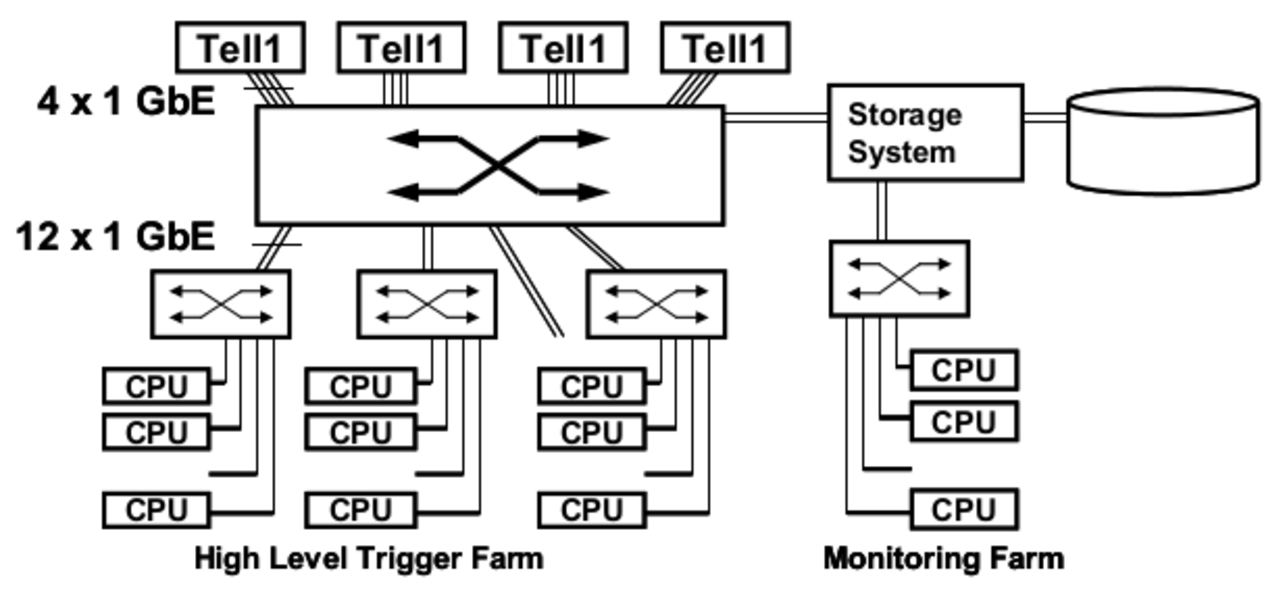
\includegraphics[height=\textheight,width=.8\textwidth, keepaspectratio=true]{figs/monitorHardWare}}\par
\end{figure}

\begin{figure}
\caption{\textit{The flow of the monitoring information.}\cite{Callot:1177133}}
\centering
\fbox{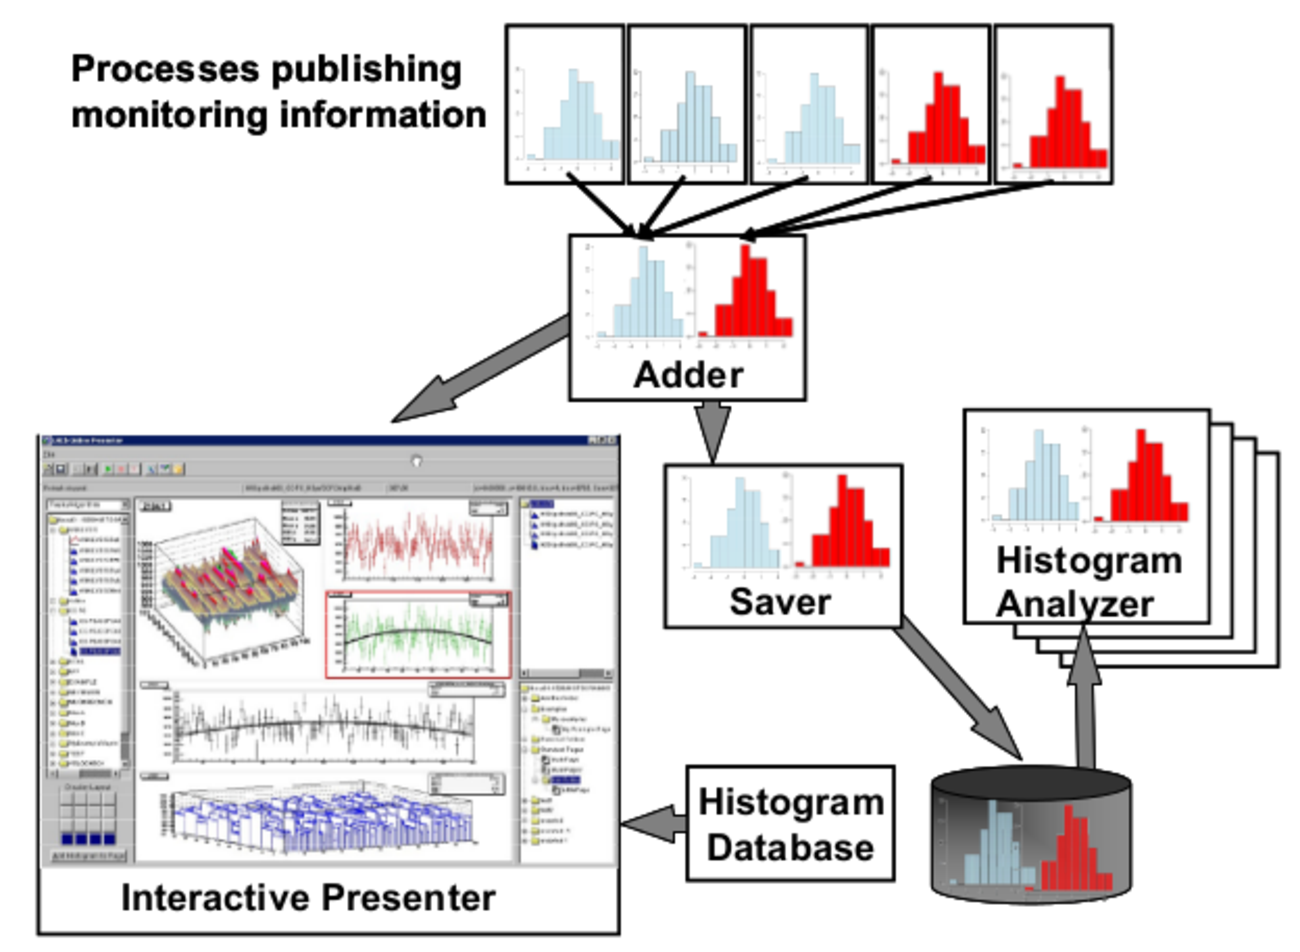
\includegraphics[height=\textheight,width=.8\textwidth, keepaspectratio=true]{figs/monitorInfoFlow}}\par
\end{figure}


\subsection{\textbf{HLT1 monitoring}}

\subsubsection{\textbf{HltMonitor.cpp}}
\subsubsection{\textbf{Introduction}}
The program flow follows the basic pattern of execution inside \textit{Gaudi}~:
initialization (\textit{initialize()}), execution ({\textit{execute()}}) and finalization ({\textit{finalize()}}). The execution method invokes all the actual monitoring methods.\par
First, some key objects present in the monitoring code will be presented and the description of the program flow will follow.\par
The first part of the documentation refers to the source file \textit{HltMonitor.cpp} found in \textit{VanDerMeer\_v6r1/Monitor/HltMonitor/src}.

\subsubsection{\textbf{RawEvent,routing bits and other key objects in monitoring}}

The \textit{RawEvent} can be considered as a persistent form of event storage containing packed and optimised data as close as possible to the detector's output. These packed data are called \textit{RawBanks} and are of many different types depending on the subdetector \cite{rawEv}.One of these banks is the ODIN RawBank,which contains information about the identity, the source and the quality of an event \cite{odin}.\par
The \textit{routing bits} can be read off a \textit{RawEvent} object and are bits set by the Trigger according to what should happen to the event after the processing in the event filter farm \cite{hlteff}.\par
The class \textit{LHCb::HltDecReports} is the container of the HLT Trigger Decision Reports. It contains the Trigger Configuration Key (TCK) used for the configuration, the Decision Reports keyed by the trigger decision name and methods for manipulating the container \cite{hltdec}.The \textit{HltDecReports} are persisted as a RawBank in RawEvent.\par

\subsubsection{\textbf{Helper methods and member variables}}
\begin{itemize}
\item \textit{monitorRoutingBit(int bit)}~: this method takes as argument a bit and checks whether it has fired or not.First it acquires a RawEvent object from which it will then extract a vector containing all the bits that have fired, which will be examined for the specific bit we want to check. The raw event is acquired from the list of possible locations of the RawEvent object in the transient store, which are ``pRec/DAQEvent'' and ``DAQ/RawEvent'' unless otherwise given in the options.\par
\item \textit{bookHlt1Histos(),bookHlt2Histos()}~: these methods first identify if there are any HLT1 error histogramms to be saved (based on the decision reports) and if yes, they book them. Note that only the histogram booking is done here, the filling is done inside the monitoring methods.\par
\item \textit{monitorErrors()}~:This method fills the error histogramms of HLT 1 and 2.It starts by checking for the decision reports.If they are found and acquired (\textit{if (decReports!=0)}), the methods for booking the HLT 1 and 2 histograms are called.When the histogram booking is over, we loop over the HLT lines filling the histogramms. The filling is done with the \textit{fill()} method of the \textit{AIDA::IHistogram1D} interface, which takes as argument a value and the corresponding weight.\cite{aida1D}.\par
\item \textit{handle()}~:This method is used during initialization to initialize certain variables as if there was a run change or the beginning of a new run.Normally the incident service (\textit{IncidentSvc}) will notify the monitoring program about the run change.\par
\item The method \textit{ODINgpsTime()} returns the time in minutes since 1970. It is received via the Beam Synchronous Timing system to allow correlating the physics events to slow control events \cite{odin}.\par  
\item \textit{updateCondition()}~:used to update the conditions from the Conditions database.\par
\item \textit{m\_nbofcollbunches}~:the number of colliding bunches, if it is greater than 0.It is used for the monitoring of the filling scheme.\par
\item \textit{m\_startEvent}~:the time at which an event took place.\par
\item \textit{m\_startClock}~:start measuring the time at the beginning of each new run.\par
\item \textit{timeset}~:shows whether or not the clock has started, that is whether the variable \textit{m\_startClock} has been initialized.It is used for the monitoring of the filling scheme.\par



\end{itemize}

\subsubsection{\textbf{Initialization,Execution and Finalization}}
\begin{itemize}
\item \label{sec:init1} The \textit{initialize()} method begins by checking whether or not we run in ``PassThrough'', that is without HLT decision reports (\textit{if (m\_hlttype.substr(0,11)=="PassThrough")}). If we do, the method returns \textit{StatusCode::SUCCESS} without further action, otherwise we proceed with the initialization of the algorithm by calling the corresponding method of the base class (\textit{GaudiHistoAlg::initialize()}).\par
Then we retrieve the Trending tool which is used to store time dependent information in an efficient way, so that it can be retrieved and displayed by the Presenter (\cite{trend}).The file name (\textit{trendname}) has to be specified using the \textit{partition} member variable which is retrieved from the JobOptions file (handled by the Application Manager, see \cite{mato1998gaudi}).\par
Next, it is checked whether or not the trigger decisions are of the same number as the histograms.If not, an exception is thrown and \textit{StatusCode::FAILURE} is returned. If yes, we proceed to build the wrapper(\ref{sec:histWrap}) for each histogram, and the tags that are needed by the Trending tool.After having built the wrappers, the histograms are booked and the underlying ROOT object of each histogram is extracted from the AIDA pointer.\par
Following the histogram booking is the registration to the \textit{IncidentSvc}, so that the monitoring program is notified everytime one of the following events occurs : start of an Event, start of a Run or Run Change. Using the \textit{handle()} method the member variables \textit{m\_startEvent,m\_startClock} and \textit{m\_currentTime} are initialized as if there was a ``Run Change'' or ``Begin Run'' event.\par
Finally, the conditions are updated from the conditions database (\textit{CondDB}) and the histogram file that was created is opened for writing.\par

\item The \textit{execute()}  method is where the monitoring methods are called. Again, if we run in ``Pass through'' mode (\textit{if (m\_hlttype.substr(0,11)=="PassThrough")}) then the method returns successfully without calling any monitoring method.Next it proceeds to call the monitoring methods \textit{LumiSeenByJob()} and \textit{monitorMu()}. At this point if the event is lumi-exclusive the \textit{execute()} method will return successfully, otherwise it will move on to invoke the rest of the monitoring methods.\par

\item The \textit{finalize()} method is called when the execution of the algorithm ends.It starts by deleting the histogram wrappers and then it closes the trending file containing the histograms.Finally, the inherited from the base class \textit{finalise()} method is called to finalize the execution of the algorithm.\par
 
\end{itemize}

\subsubsection{\textbf{Monitoring functions}}\label{sec:hlt1methods}
\begin{itemize}
\item \textit{monitorVertices()}~:Provided there are available vertex reports this method fills the monitoring histograms for the vertices, as well as the corresponding profile histograms.Profile histograms are used to display the mean value of the Y axis and its error for each bin in the X axis.\par
\item \textit{monitorMasses()}~:Provided there are HLT selection reports available, this method fills the mass plots through each histogram wrapper.\par
\item \textit{MonitorMu()}~:This method begins by acquiring the ODIN RawBank from which we will check the source of the trigger and the bunch crossing type (\textit{if ( ( odin-$>$triggerType() == LHCb::ODIN::LumiTrigger ) && ( odin-$>$bunchCrossingType() == LHCb::ODIN::BeamCrossing ) )} respectively).If the trigger type is random trigger (\cite{odin_bank})  and the bunch crossing type (\textit{BXtype}) is beam crossing then we proceed to find the fraction of empty events, which are equally important to calculate the luminosity as the selected events \cite{lumiCnt}.\par
If the lumi counter \textit{m\_Counter} has the value corresponding to a random method (value == 21) we proceed to examine the \textit{HltLumiSummary} (\cite{lumiXML}).\par
After checking that an \textit{HltLumiSummary} RawBank exists, the method proceeds to acquire it and extract the information stored in it (\textit{hltLumiSummary-$>$extraInfo()}, see \cite{lumiSum}).Based on this information, the method fills the \textit{m\_lumi\_rate} or the  \textit{m\_lumi\_ee\_rate} histograms.The execution concludes with the filling of the \textit{m\_mu\_rate\_root} histogram.\par
\item \textit{LumiSeenByJob}~:This method follows the same execution pattern as \textit{MonitorMu()}, but fills the \textit{m\_total\_lumi\_rate} histogram.\par


\end{itemize}


\subsection{\textbf{HistoWrapper.cpp}}\label{sec:histWrap}
\subsubsection{\textbf{Introduction}}
\textit{HistoWrapper} is a simple wrapper class which contains information about histograms.\par

\subsubsection{\textbf{Methods}}
\begin{itemize}
\item \textit{HistoWrapper()}~:The default constructor initializes the variables and books the following histograms for each measured quantity~:\textit{invariant mass,left,center,right,tmp,rate per 10^6 pp interactions, mass vs SPD hits,signaloverbg,chi2perdof,chi2perdof\_bg,pT}.\par
\item \textit{fill(const LHCb::HltSelReports* selReports, double when, AIDA::IHistogram1D* m\_total\_lumi\_rate, double scale ,AIDA::IHistogram1D* m\_mu\_rate, int SPDmultiplicity )}~: First we check if the variables \textit{m\_massDef} and \textit{m\_rateDef} contain all the necessary information (have the correct size - \textit{if ( m\_massDef.size() != 5 $||$ m\_rateDef.size() != 3 )}.Next, we check if the trigger decision name (\textit{m\_decision}) is present in the container \textit{selReports} (\textit{if ( !selReports-$>$hasSelectionName( decision() ) )}). If it is not, the method returns, otherwise it proceeds to acquire a pointer to the HLT selection report for the given trigger decision name~: \textit{selReport = selReports-$>$selReport( decision() )}.Then, we loop over all the objects on which the selection report was built and fill in the previously booked histograms.(\cite{hltobjectsum}).\par
\item \textit{getBinContent()}~:gets the content of the previous bin.\par

\end{itemize}

\subsection{\textbf{ErrorHistoWrapper.cpp}}
\subsubsection{\textbf{Introduction}}
\textit{ErrorHistoWrapper} is a simple wrapper class which contains information about error histograms.It is based on the previously discussed \textit{HistoWrapper} class.\par


\subsubsection{\textbf{Methods}}
\begin{itemize}
\item \textit{ErrorHistoWrapper()}~:The constructor takes the necessary steps to initialize the HLT2 error histograms (book them, set axes, labels).\par
\item \textit{fill()}~:It fills the error histograms for each of the HLT2 lines.\par

\end{itemize}

\subsection{\textbf{HltTupleMaker.cpp}}
\subsubsection{\textbf{Introduction}}
\textit{HltTupleMaker} is a simple algorithm which puts some event info,Hlt2 candidate masses and occupancies in an ntuple. As a Gaudi algorithm it follows the usual execution pattern : initialize, execute, finalize.\par

\subsubsection{\textbf{Methods}}
\begin{itemize}
\item \textit{initialize()}~:The Algorithm subscribes itself to the \textit{IIncidentSvc}, to be notified of a run change or the beginning of a new run.Next we fill the \textit{m\_occupancies} container with the required occupancy methods and acquire the \textit{OTRawBankDecoder} tool.The occupancy methods are~: \textit{OTOccupancy()}, which returns the total number of hits in the Outer Tracker without decoding the modules.This is useful in pattern recognition to remove the full events; \textit{ITClusters()},which returns the size of the Silicon Tracker LiteClusters; \textit{VeloClusters}, which return the size of the VELO LiteClusters and \textit{SPDMultiplicity()}, which extracts information from the Level-0 decision unit report (\textit{L0DUReport}) .\par
\item \textit{execute()}~:The \textit{execute} method retrieves event information from the ODIN raw bank and then continues to acquire the HLT decision and selection reports.\par
\item \textit{finalize()}~:In this method open files are closed and pointers are deleted before finalising the Algorithm through the base class method (\textit{GaudiAlgorithm::finalize()}).\par
\item \textit{createFile()}~:It creates the tuple file we want to process. If the directory of the file is not there, we create it; if the file already exists, we open it with an \textit{``update''} flag.\par
\item \textit{createTree()}~:The method starts with inserting the candidate masses into the corresponding member variable (\textit{m\_masses}).Next, it continues to build the tree setting the masses and the occupancies to its branches.The way of building the tree depends on whether the tree exists or not; in the first case we re-point the branches to their new contents (see \cite{ttree}).\par
\item \textit{fillTree()}~:This method fills in the tree with the required information~:masses, acquired from selection reports, occupancies and routing bits.\par


\end{itemize}


\subsection{\textbf{HltMuonAsymMonitor.cpp}}

\subsubsection{\textbf{Introduction}}
The execution flow of the \textit{HltMuonAsymMonitor} follows the same pattern as every Gaudi Algorithm~: \textit{initialize(), execute()} and \textit{finalize()}.\par
\subsubsection{\textbf{Methods}}.
\begin{itemize}
\item \textit{initialize()}~:The nethod starts by initializing the Algorithm using the base class initialization method.It then proceeds by booking the histograms,filling the Look-up Tables (LUT) and checking to make sure that the LUT will be filled and saved successfully.\par
\item \textit{execute()}~:First we try to retrieve the L0DU report, the L0Muon candidates and the selection reports.To acquire the selection reports we have to have set the \textit{m\_decision} member variable in the options.Finally, we retrieve the corresponding report for the decision, get the run number from the ODIN raw bank and call the monitoring method \textit{monitorAsym()} with the L0Muon candidates and the selection report as arguments.\par
\item \textit{finalize()}~:In the finalization, we save the LUT and finalize the Algorithm using the base class method.\par
\item \textit{monitorAsym()}~:In this method first we acquire the first HLT candidate and fill the J/Psi mass histogram.Then we loop over its daughters and their tracks and check for matches between muons and L0 candidates.Finally we loop over the muon pairs examining them and filling the necessary histograms.\par

\end{itemize}

\subsubsection{\textbf{Helper methods}}
There are special methods for handling LUTs (\textit{openLUT,fillLut,getPTFromLUT,writeLUT}), as well as for getting the candidate M1 and M2 pads (\textit{getCandidatePads}) and the time (\textit{getTime()}).\par


\subsection{\textbf{HLT2 monitoring}}

\subsubsection{\textbf{HltMassMonitor.cpp}}
\subsubsection{\textbf{Introduction}}
The execution of the HLT 2 monitoring program is very similar to the corresponding for HLT 1.It follows the usual pattern: \textit{initialization,execution,finalization}.

\subsubsection{\textbf{Methods}}

\begin{itemize}
\item \textit{initialize()}~:same as for HLT1 monitor, see \ref{sec:init1}.
\item \textit{execute()}~:same as for HLT1 monitor (see \ref{sec:init1}), but now we just monitor the masses and Mu (not errors or vertices).\par
\item \textit{finalize()}~:clears the wrappers and finalizes the Algorithm  (see \ref{sec:init1}).\par

\end{itemize}

\subsubsection{\textbf{Monitoring methods}}
Most of the monitoring functions used in HLT 2 are the same as HLT 1 except for a few additions (\ref{sec:hlt1methods}).\par

\begin{itemize}

\item \textit{monitorMasses()}~:Add the signal-to-background ratio to the histogram as well (apart from rate).\par
\item \textit{monitorMu()}~:Same as HLT 1, but the content of one more bin is added to the \textit{m\_mu\_rate\_root} histogram (\textit{m\_trend-$>$addValue( std::string("Mu") , m\_mu\_rate\_root-$>$GetBinContent(now-1))}).\par

\end{itemize}

